\clearpage
\section*{Question 5}
\addcontentsline{toc}{section}{Question 5}

Analyze the stability of the Forward Euler (ode1) and explicit RK5 (ode5) methods for the RLC circuit. Plot the stability regions and indicate the range of $h$ for which the methods are stable. \\ 

\subsection*{Stability Plots}
The following figure shows the stability regions for Forward Euler (ode1) and explicit RK5 (ode5) methods, with the scaled eigenvalues $z = h \lambda$ plotted for various step sizes $h$:
\begin{figure}[H]
	\centering
	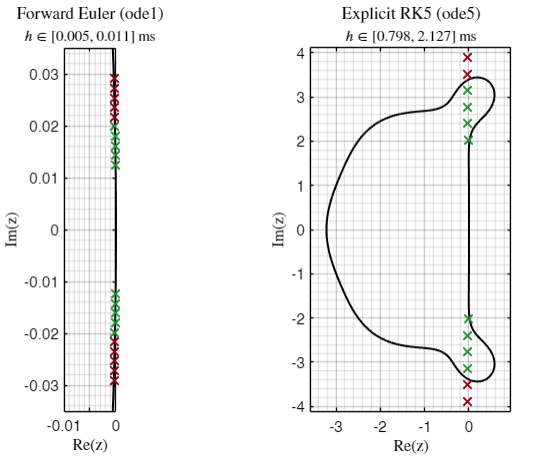
\includegraphics[width=0.95\textwidth]{figures/hw01_q05_fe-rk5-stabilty-regions-with-candidate-step-values.png}
	\caption{Stability regions for Forward Euler (ode1, left) and explicit RK5 (ode5, right). Each cross represents $z = h \lambda$ for a candidate step size $h$ and the system eigenvalues $\lambda$. Green crosses are inside the stability region (stable), red crosses are outside (unstable). Note that the plot for Forward Euler is zoomed in to show the small stability region.}
\end{figure}

\subsection*{Stability Criteria and $z$ Formulae}
For a linear system $\dot{x} = \lambda x$, the stability of a numerical method is determined by the location of $z = h \lambda$ in the method's stability region:
\begin{itemize}
	\item \textbf{Forward Euler (FE):} The stability function is $R(z) = 1 + z$. The method is stable if $|1 + z| < 1$.
	\item \textbf{Explicit RK5 (Taylor-5):} The stability function is $R(z) = 1 + z + \frac{z^2}{2!} + \frac{z^3}{3!} + \frac{z^4}{4!} + \frac{z^5}{5!}$. The method is stable if $|R(z)| < 1$. (Note: MATLAB's ode5 is not exactly a Taylor-5 method, but the Taylor-5 region is a good approximation for illustration.)
\end{itemize}

\subsection*{Interpretation of Crosses}
Each cross in the plot corresponds to a value of $z = h \lambda$ for a particular step size $h$ and one of the system's eigenvalues $\lambda$. \\ 
	\textbf{Green crosses} indicate $z$ values inside the stability region (method is stable for that $h$), while \textbf{red crosses} are outside (unstable for that $h$).

\subsection*{Maximum Stable Step Size}
From the plot and MATLAB output:
\begin{itemize}
	\item \textbf{Euler:} $h_\text{max} \approx 0.008$ ms
	\item \textbf{Taylor-5:} $h_\text{max} \approx 1.329$ ms
\end{itemize}
These values indicate the largest time step for which each method remains stable for the given system.

\subsection*{Summary}
The explicit RK5 (Taylor-5) method allows for a much larger stable time step than Forward Euler, as seen from the much larger stability region. The actual ode5 implementation in MATLAB is not exactly Taylor-5, but the qualitative stability behavior is similar for this analysis.


